\chapter{Introduction}
\label{introduction}

Much of the recent history of genome editing consists of building the site-specificity of a nuclease through engineered protein-DNA interactions. Though this technique has proven effective and useful, as seen in the examples of Zinc-Finger Nucleases (ZFNs) and Transcription Activator-Like Effector Nucleases (TALENs), these platforms are difficult to use because of the complexity of programming protein-DNA specificity.
In recent years, the CRISPR-Cas bacterial immune system has been extensively used as a genome engineering alternative that relies on RNA-DNA complementarity as the homing interaction that guides the specificity of the Cas9 nuclease. The ease of using such a platform to cleave specific sites in the genome simply by choosing a guide RNA sequence complementary to the target sequence has lead to an explosion in its use, with enormous amounts of interest and capital being contributed to the investigation of further development and application of this technology (Doudna and Charpentier \textit{et al.} 2014).

In what is perhaps the most important paper in the field, the Doudna (UC Berkeley) and Charpentier (Umea University, Sweden) labs teamed up in 2012 to fully characterize the homing mechanism of the Cas9 nuclease. Through exclusively \textit{in vitro} assays, they found that Cas9, the tracrRNA, the crRNA with a spacer specifying the correct target, and magnesium ions, are all that is needed for cleavage of target DNA to occur. They further validated that complementarity between the spacer and the target is necessary for cleavage, and that one or two mismatches in this spacer::target complementarity is tolerated. Additionally, they showed that cleavage of a target depends on a ``protospacer adjacent motif" (PAM) sequence, which is specified by the Cas9 protein, not the spacer (Jinek and Chylinski \textit{et al.} 2012).

\begin{figure}[!h]
	\begin{center}
	\centerline{
	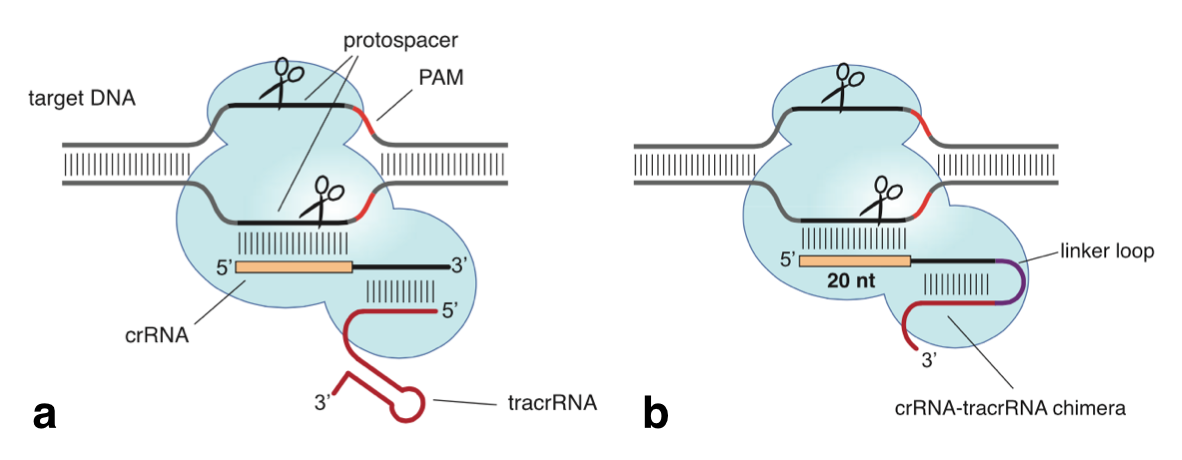
\includegraphics[width=1.15\textwidth]{figures/grna.png}
	}
	\caption{An RNA complex guides Cas9 to its target. \textbf{(a)} The matured crRNA and tracrRNA complex to guide Cas9. \textbf{(b)} A single gRNA comprising of the crRNA, a linker loop, and a crRNA guides Cas9 with the same efficiency as the dual-guide system. (Adapted from Jinek and Chylinski \textit{et al.} 2012)}
	\label{fig:grna}
	\end{center}
\end{figure}

Finally, realizing that the CRISPR-Cas system could be an easily programmable nuclease, the authors constructed a synthetic platform that marked the first time that this system was engineered for easier biotechnological use. They fused the tracrRNA and crRNA sequences (as they would be after maturation by RNAseIII) together with a short linker loop and expressed the entire construct as a single sequence. This led to very strong cleavage, indicating that bypassing the maturation step increases the activity of CRISPR-Cas restriction. This fused RNA molecule concept, dubbed the guide RNA (gRNA) is now nearly universally used in all applications of the CRISPR-Cas platform.

The findings of Jinek and Chylinski \textit{et al.} (2012) kicked off a frenzy of development for the CRISPR-Cas9 platform, but also made researchers more curious about the nature of this system and how it is used by bacteria in the wild. Now that the mechanisms of specificity and restriction had been elucidated, the last question was how the system adapted to pathogens through the integration of new spacer sequences in the CRISPR array.

%
%The molecular basis of Cas9 specificity comes from two independent RNA sequences: the CRISPR RNA (crRNA) and the transactivating CRISPR RNA (tracrRNA). In the wild, the tracrRNA and crRNA complex at a region of complementarity, are processed by endogenous nonspecific exonucleases, and then associate with Cas9 for a final crRNA-tracrRNA-Cas9 complex. When using the system in the lab, the crRNA and the tracrRNA are expressed as a single guide RNA (gRNA) strand to simply the formation of the final RNA-Protein complex. Cas9 then scans genomic DNA for a short Protospacer-Adjacent Motif (PAM) sequence, which is hard-coded into the protein. Once a match is found, Cas9 then alters its conformation to check for complementarity between the 20 nucleotide gRNA spacer sequence and the adjacent genomic DNA. If a match is found, Cas9 then makes a double stranded break at that locus (Jinek \textit{et al.} 2012, Anders \textit{et al.} 2014).
%
%Once a double stranded break occurs in a eukaryotic cell, cellular machinery quickly repairs the break through either non-homologous end joining (NHEJ) or homology directed repair (HDR). In the case of NHEJ, random blunt end resections or small nucleotide insertions can occur, causing a deletion or insertion of one or more nucleotides in the final repaired site. This is phenomenon is often used to induce frame-shift mutations into a gene to  knock it out. In the case of HDR, a donor strand of DNA is used to template a precise insertion at the site of repair (Doudna and Charpentier 2014).
%
%Perhaps one of the largest questions in the CRISPR-Cas9 field is that of targetability. Since there is a PAM sequence requirement for all known Cas9 proteins, each can only target a limited subset of all possible genomic targets. Interestingly, since the CRISPR-Cas system evolved as a bacterial immune system against viral DNA, and since different bacterial strains are attacked by vastly different phages, the Cas9 proteins from different strains seem to have differing PAM specificities. Thus, the targeting range of the CRISPR-Cas platform can be expanded by adding more Cas9s to choose from (Kleinstiver \textit{et al.} 2015).
%
%Of similar import is specificity. Because RNA and DNA can form complementary complexes even in the presence of a small number of mismatches between the two molecules' sequences, CRISPR-Cas9 often cleaves at off-target locations in a generally unpredictable manner. This has huge implications in applications of CRISPR-Cas9, as off-target activity can possibly have catastrophic effects on a cell. We have recently described an assay for detecting off-target cleavage events by Cas9 in an unbiased manner, which can be used to better understand the specificities of different Cas9 proteins (Tsai \textit{et al.} 2015).